
\documentclass{beamer}
\usecolortheme{dove}
\setbeamertemplate{navigation symbols}{}
\usepackage{amsmath,amssymb,amsfonts,amsthm, multicol, subfigure, color}
\usepackage{bm}
\usepackage{graphicx}
\usepackage{tabularx}
\usepackage{booktabs}
\usepackage{hyperref}
\usepackage{pdfpages}
\usepackage{xcolor}
\definecolor{seagreen}{RGB}{46, 139, 87}
\def\independenT#1#2{\mathrel{\rlap{$#1#2$}\mkern2mu{#1#2}}}
\newcommand\indep{\protect\mathpalette{\protect\independenT}{\perp}}
\def\log{\text{log}}
\newcommand\logit{\text{logit}}
\newcommand\iid{\stackrel{\text{iid}}{\sim}}
\newcommand\E{\text{E}}
\newcommand\V{\text{V}}
\renewcommand\P{\text{P}}
\newcommand{\Cov}{\text{Cov}}
\newcommand{\Cor}{\text{Cor}}
\newcommand\doop{\texttt{do}}
\usepackage{stackrel}
\usepackage{tikz}
\usetikzlibrary{arrows,shapes.arrows,positioning,shapes,patterns,calc}
\newcommand\slideref[1]{\vskip .1cm \tiny \textcolor{gray}{{#1}}}
\newcommand\red[1]{\color{red}#1}
\newcommand\blue[1]{\color{blue}#1}
\newcommand\gray[1]{\color{gray}#1}
\newcommand\seagreen[1]{\color{seagreen}#1}
\newcommand\purple[1]{\color{purple}#1}
\newcommand\orange[1]{\color{orange}#1}
\newcommand\black[1]{\color{black}#1}
\newcommand\white[1]{\color{white}#1}
\newcommand\teal[1]{\color{teal}#1}
\newcommand\magenta[1]{\color{magenta}#1}
\newcommand\Fuchsia[1]{\color{Fuchsia}#1}
\newcommand\BlueGreen[1]{\color{BlueGreen}#1}
\newcommand\bblue[1]{\textcolor{blue}{\textbf{#1}}}
\newcommand\bred[1]{\textcolor{red}{\textbf{#1}}}
\newcommand\bgray[1]{\textcolor{gray}{\textbf{#1}}}
\newcommand\bgreen[1]{\textcolor{seagreen}{\textbf{#1}}}
\newcommand\bref[2]{\href{#1}{\color{blue}{#2}}}
\colorlet{lightgray}{gray!40}
\pgfdeclarelayer{bg}    % declare background layer for tikz
\pgfsetlayers{bg,main} % order layers for tikz
\newcommand\mycite[1]{\begin{scriptsize}\textcolor{darkgray}{(#1)}\end{scriptsize}}
\newcommand{\tcframe}{\frame{
%\small{
\only<1|handout:0>{\tableofcontents}
\only<2|handout:1>{\tableofcontents[currentsection]}}
%}
}

\usepackage[round]{natbib}
\bibliographystyle{humannat-mod}
\setbeamertemplate{enumerate items}[default]
\usepackage{mathtools}

\newcommand{\goalsframe}{\begin{frame}{Learning goals for today}
At the end of class, you will be able to:
\begin{enumerate}
\item Encode causal theories in Directed Acyclic Graphs (DAGs)
\item Identify causal effects by blocking backdoor paths
\item Understand collider variables
\end{enumerate} \vskip .2in
\end{frame}}

\title{5. Exchangeability: Assumptions to block backdoor paths}
\author{Ian Lundberg\\Cornell Info 6751: Causal Inference in Observational Settings\\Fall 2022}
\date{6 Sep 2022}

\begin{document}

\maketitle

\goalsframe

\begin{frame}{What is a \bblue{Directed Acyclic Graph (DAG)}?}\pause

A DAG is a formal graph, used for causal assumptions\pause
\begin{itemize}
\item Each \bblue{node} is a variable
\item Each \bblue{edge} is a causal relation
\end{itemize}

\begin{center}
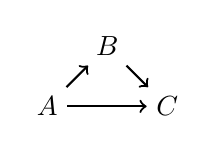
\begin{tikzpicture}[x = .3in, y = .3in]
\node (a) at (0,0) {$A$};
\node (b) at (1,1) {$B$};
\node (c) at (2,0) {$C$};
\draw[->, thick] (a) -- (b);
\draw[->, thick] (b) -- (c);
\draw[->, thick] (a) -- (c);
\end{tikzpicture}
\end{center} \pause
What makes it a DAG? \pause It is directed and acyclic.
\begin{itemize}
\item Directed: Every edge has an arrow. Causality flows one way.
\item Acyclic: There are no cycles
\end{itemize}
\begin{center}

\begin{tikzpicture}[x = .25in, y = .3in]
\node[font = \footnotesize] (a) at (0,1) {};
\node[font = \footnotesize] (b) at (1,-.8) {};
\node[red] (c) at (.5,.5) {Not DAGs:};
\end{tikzpicture}
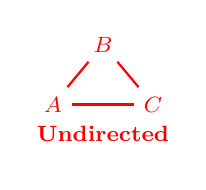
\begin{tikzpicture}[x = .25in, y = .3in]
\node[font = \footnotesize, red] (a) at (0,0) {$A$};
\node[font = \footnotesize, red] (b) at (1,1) {$B$};
\node[font = \footnotesize, red] (c) at (2,0) {$C$};
\draw[thick, red] (a) -- (b);
\draw[thick, red] (b) -- (c);
\draw[thick, red] (c) -- (a);
\node[red, font = {\bf\footnotesize}, anchor = north] at (1,-.2) {Undirected};
\node[font = \footnotesize] (b) at (1,-.8) {};
\end{tikzpicture}
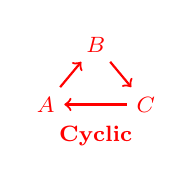
\begin{tikzpicture}[x = .25in, y = .3in]
\node[font = \footnotesize, red] (a) at (0,0) {$A$};
\node[font = \footnotesize, red] (b) at (1,1) {$B$};
\node[font = \footnotesize, red] (c) at (2,0) {$C$};
\draw[->, thick, red] (a) -- (b);
\draw[->, thick, red] (b) -- (c);
\draw[->, thick, red] (c) -- (a);
\node[red, font = {\bf\footnotesize}, anchor = north] at (1,-.2) {Cyclic};
\node[font = \footnotesize] (b) at (1,-.8) {};
\end{tikzpicture}
\end{center}

\end{frame}

\begin{frame}{Why draw a DAG? Four reasons} \pause

\begin{enumerate}[<+->]
\item DAGs formalize the theory we believe before we see any data
\item DAGs often formalize things the data cannot tell us
\item DAGs are mathematically precise, with formal properties
\item DAGs are intuitive
\end{enumerate}

\end{frame}

\begin{frame}{1) Completely randomized experiment}\pause

Flip a coin. Assign job training. Observe employment. \pause
\vskip .2in

\begin{center}
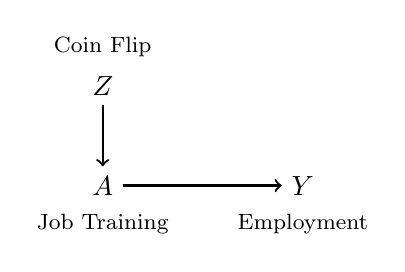
\begin{tikzpicture}[x = 1in, y = .5in]
\node[align = center] (z) at (0,1) {$Z$};
\node[font = \footnotesize, align = center, anchor = south] (zlab) at (z.north) {Coin Flip};\pause
\node (a) at (0,0) {$A$};
\node[anchor = north, font = \footnotesize] at (a.south) (0,0) {Job Training};
\draw[->, thick] (z) -- (a);\pause
\node (y) at (1,0) {$Y$};
\draw[->, thick] (a) -- (y);
\node[anchor = north, font = \footnotesize] at (y.south) (0,0) {Employment};
\end{tikzpicture} 
\end{center} \vskip .2in 
\onslide<6->{Recall: Heads and tails are \bblue{exchangeable}.}
\end{frame}

\begin{frame}{2) Randomized experiment: Unequal probabilities} \pause

Assign job training with higher probability\\to those who were not employed last year.\vskip .2in \pause
\begin{center}
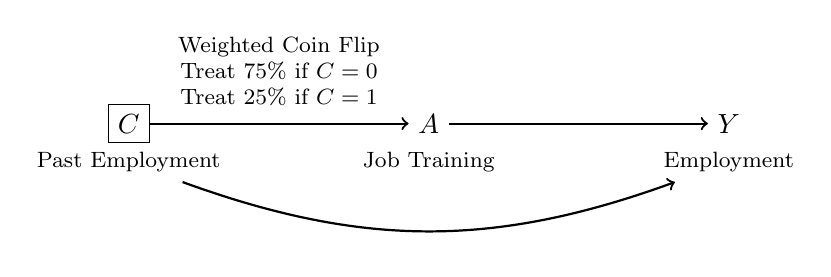
\begin{tikzpicture}[x = 1.5in, y = .5in]
\node[align = center] (c) at (-1,0) {$C$};
\node (a) at (0,0) {$A$};
\node (y) at (1,0) {$Y$};
\node[anchor = north, font = \footnotesize] (alab) at (a.south) (0,0) {Job Training};
\node[anchor = north, font = \footnotesize] (ylab) at (y.south) {Employment};
\node[font = \footnotesize, align = center, anchor = north] (clab) at (c.south) {Past Employment};
\draw[->, thick] (c) -- node[midway, above, align = center, font = \footnotesize, outer sep = 3pt] {Weighted Coin Flip\\Treat 75\% if $C = 0$\\Treat 25\% if $C = 1$} (a);
\draw[->, thick] (a) -- (y);
\draw[->, thick] (clab) to[bend right = 20] (ylab);
\draw<5-> (c.south west) rectangle (c.north east);
\end{tikzpicture}
\end{center}
\vskip .2in \pause
\begin{tabular}{ll}
\bgray{Question:} & How can we analyze data from this experiment? \pause\\
\bgray{Answer:} & We should analyze within subgroups of $C$\pause \\
& Heads and tails are \bblue{conditionally exchangeable} \pause \\
\bgray{Next up:} & Formalize this intuition
\end{tabular}
\end{frame}

\begin{frame}{Key Concept: Backdoor Adjustment}
\pause

There are two reasons $A$ and $Y$ are associated
\begin{itemize}
\onslide<3->{\item A \bblue{causal path} $A\rightarrow Y$}
\onslide<4->{\item A \bred{backdoor path} $A \leftarrow C\rightarrow Y$}
\begin{itemize}
\onslide<5->{\item Think of a house at $A$}
\onslide<6->{\item Walk out the back door to $C$, then around the house to $Y$}
\end{itemize}
\end{itemize}
\begin{center}
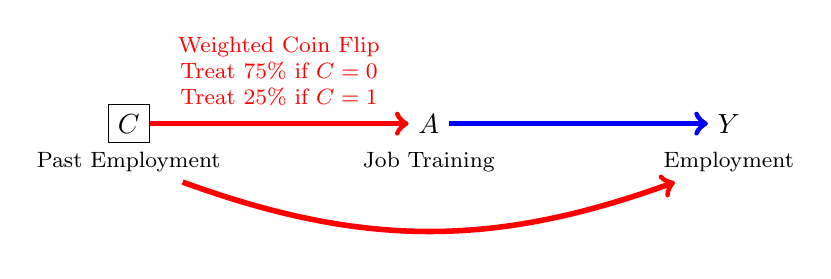
\begin{tikzpicture}[x = 1.5in, y = .5in]
\onslide<3->{
\node (a) at (0,0) {$A$};
\node (y) at (1,0) {$Y$};
\node[anchor = north, font = \footnotesize] (alab) at (a.south) (0,0) {Job Training};
\node[anchor = north, font = \footnotesize] (ylab) at (y.south) {Employment};
\draw[->, line width = 2pt, blue] (a) -- (y);
}
\onslide<4->{
\node[align = center] (c) at (-1,0) {$C$};
\node[font = \footnotesize, align = center, anchor = north] (clab) at (c.south) {Past Employment};
\draw[->, line width = 2pt, red] (c) -- node[midway, above, align = center, font = \footnotesize, outer sep = 3pt] {Weighted Coin Flip\\Treat 75\% if $C = 0$\\Treat 25\% if $C = 1$} (a);
\draw[->, line width = 2pt, red] (clab) to[bend right = 20] (ylab);
}
\draw<9-> (c.south west) rectangle (c.north east);
\end{tikzpicture}
\end{center}
\onslide<7->{To block the backdoor path, condition on $C$}
\begin{itemize}
\onslide<8->{\item Analyze within strata of $C$}
\onslide<9->{\item Denoted by the box}
\end{itemize}
\end{frame}

\begin{frame}{Check: The power of backdoor adjustment} \pause

\begin{itemize}[<+->]
\item If my DAG is true
\item and I adjust for the required variables
\item then my observational data support a causal claim\\(just like an experiment would)
\end{itemize} \pause
Only difference: In an experiment we know the DAG is true.

\end{frame}

\begin{frame}{Key Concept: Causal Identification}
\onslide<2->{
\begin{tabular}{rl}
Causal identification links\\
causal quantities &(involving potential outcomes, e.g. $Y^a$)\\
to statistical quantities &(involving observable variables, e.g. $Y$)
\end{tabular}
}
\begin{center}
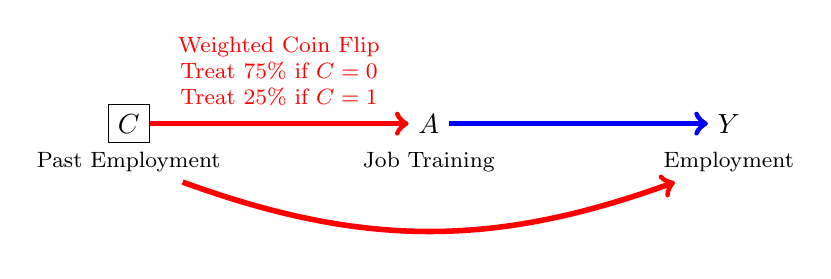
\begin{tikzpicture}[x = 1.5in, y = .5in]
\node[align = center] (c) at (-1,0) {$C$};
\node (a) at (0,0) {$A$};
\node (y) at (1,0) {$Y$};
\node[anchor = north, font = \footnotesize] (alab) at (a.south) (0,0) {Job Training};
\node[anchor = north, font = \footnotesize] (ylab) at (y.south) {Employment};
\node[font = \footnotesize, align = center, anchor = north] (clab) at (c.south) {Past Employment};
\draw[->, line width = 2pt, red] (c) -- node[midway, above, align = center, font = \footnotesize, outer sep = 3pt] {Weighted Coin Flip\\Treat 75\% if $C = 0$\\Treat 25\% if $C = 1$} (a);
\draw[->, line width = 2pt, blue] (a) -- (y);
\draw[->, line width = 2pt, red] (clab) to[bend right = 20] (ylab);
\draw (c.south west) rectangle (c.north east);
\end{tikzpicture}
\end{center}
\onslide<3->{
Once we block the backdoor path,
$$\underbrace{\E(Y^a\mid C = c)}_\text{Causal Quantity} = \underbrace{\E(Y\mid C = c, A = a)}_\text{Statistical Quantity}$$
}
\onslide<4->{
Also known as \bgray{conditional exchangeability} {\footnotesize (Hern\'an \& Robins 3.2)}
}
\end{frame}

\begin{frame}{Key Concept: Sufficient Adjustment Set}\pause

A \bblue{sufficient adjustment set} is any set of variables that blocks all backdoor paths between the treatment and outcome\vskip .1in \pause
%Example:
\begin{center}
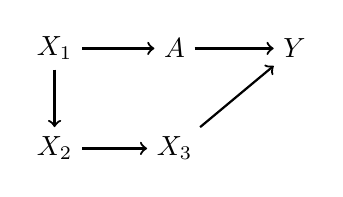
\begin{tikzpicture}[x = .6in, y = .5in]
\node (a) at (0,0) {$A$};
\node (y) at (1,0) {$Y$};
\node (x1) at (-1,0) {$X_1$};
\node (x2) at (-1,-1) {$X_2$};
\node (x3) at (0,-1) {$X_3$};
\draw[->, thick] (a) -- (y);
\draw[->, thick] (x1) -- (a);
\draw[->, thick] (x1) -- (x2);
\draw[->, thick] (x2) -- (x3);
\draw[->, thick] (x3) -- (y);
\end{tikzpicture}
\end{center} \vskip .1in \pause
We can block the backdoor path in any of 3 ways:
\begin{itemize} \pause
\item Condition on $X_1$: $A\leftarrow \boxed{X_1}\rightarrow X_2\rightarrow X_3\rightarrow Y$ \pause
\item Condition on $X_2$: $A\leftarrow X_1\rightarrow \boxed{X_2}\rightarrow X_3\rightarrow Y$ \pause
\item Condition on $X_3$: $A\leftarrow X_1\rightarrow X_2\rightarrow \boxed{X_3}\rightarrow Y$
\end{itemize}

\end{frame}

\begin{frame}{Key Concept: Colliders\footnote{Example from Pearl, J. (1988). Probabilistic Reasoning in Intelligent Systems: Networks of Plausible Inference.}} \pause

Suppose I have sprinklers on a timer. \pause
\begin{center}
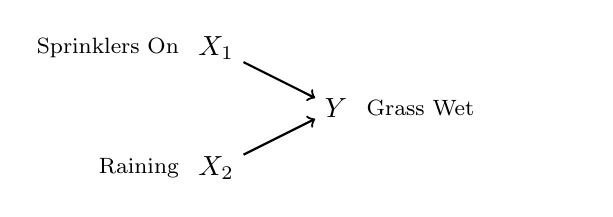
\begin{tikzpicture}[x = .6in, y = .3in]
\node at (-2,0) {};
\node at (2,0) {};
%\onslide<2->{
\node (x1) at (-1,0) {$X_1$};
\node (x2) at (0,-1) {$Y$};
\node (x3) at (-1,-2) {$X_2$};
\node[anchor = east, font = \footnotesize] at (x1.west) {Sprinklers On};
\node[anchor = east, font = \footnotesize] at (x3.west) {Raining};
\node[anchor = west, font = \footnotesize] at (x2.east) {Grass Wet};
%\draw[->, thick] (a) -- (y);
\draw[->, thick] (x1) -- (x2);
\draw[->, thick] (x3) -- (x2);
\end{tikzpicture}
\end{center} \pause
We say $Y$ is a \bblue{collider} along the path $X_1\rightarrow Y \leftarrow X_2$ \pause
\begin{itemize}
\item The collider blocks the path \pause
\item $X_1$ is independent of $X_2$
\begin{itemize}
\item (Sprinklers On) is uninformative about (Raining)
\end{itemize} \pause
\item Conditioning on $Y$ opens the path
\begin{itemize}
\item If the grass is wet (conditional on $Y = 1$),\\then either (Sprinklers On) or (Raining)
\end{itemize}
\end{itemize}
\end{frame}

\begin{frame}{Ancestors vs.~Colliders}

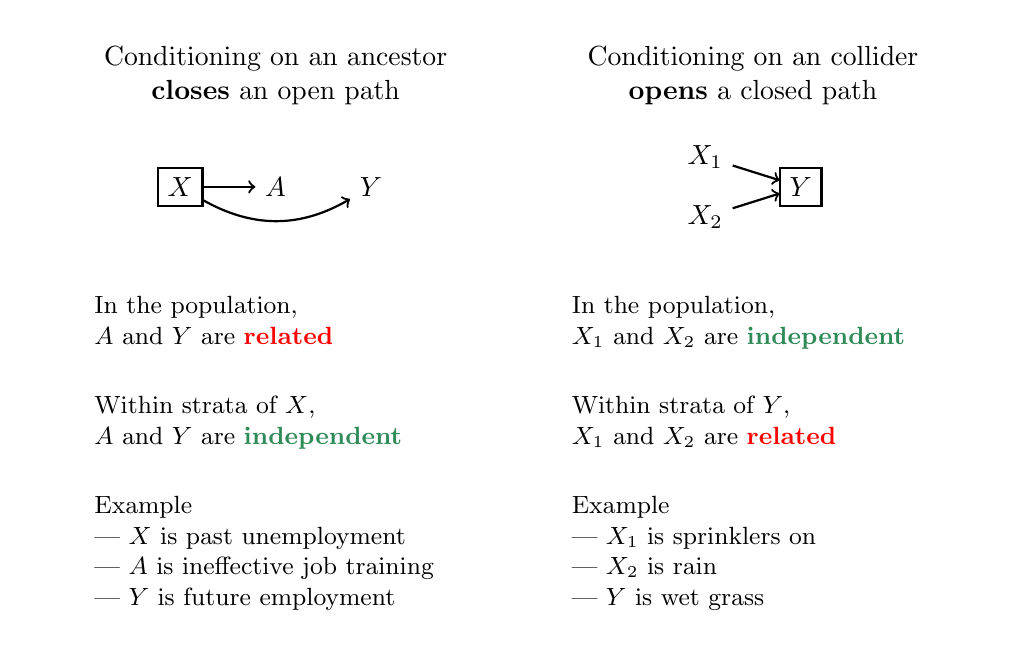
\begin{tikzpicture}[x = \textwidth, y = .5in]
\node at (0,0) {};
\node at (1,0) {};
\node[anchor = north, align = center] at (.25,0) {Conditioning on an ancestor\\\textbf{closes} an open path};
\node[anchor = north, align = center] at (.75,0) {Conditioning on an collider\\\textbf{opens} a closed path};
% ANCESTOR DAG
\node (x) at (.15,-1.5) {$X$};
\node (a) at (.25,-1.5) {$A$};
\node (ya) at (.35,-1.5) {$Y$};
\draw[thick] (x.south west) rectangle (x.north east);
\draw[->, thick] (x) -- (a);
\draw[->, thick] (x) to[bend right] (ya);
%\draw[->, thick] (a) -- (ya);
% COLLIDER DAG
\node (x1) at (.7,-1.2) {$X_1$};
\node (yc) at (.8,-1.5) {$Y$};
\node (x3) at (.7,-1.8) {$X_2$};
\draw[thick] (yc.south west) rectangle (yc.north east);
\draw[->, thick] (x1) -- (yc);
\draw[->, thick] (x3) -- (yc); \pause
% POPULATION
\node[anchor = north west, align = left, font = \small] at (.05,-2.5) {In the population,\\$A$ and $Y$ are \bred{related}}; \pause
\node[anchor = north west, align = left, font = \small] at (.55,-2.5) {In the population,\\$X_1$ and $X_2$ are \bgreen{independent}}; \pause
% STRATA
\node[anchor = north west, align = left, font = \small] at (.05,-3.5) {Within strata of $X$,\\$A$ and $Y$ are \bgreen{independent}}; \pause
\node[anchor = north west, align = left, font = \small] at (.55,-3.5) {Within strata of $Y$,\\$X_1$ and $X_2$ are \bred{related}}; \pause
% EXAMPLE
\node[font = \small, align = left, anchor = north west] at (.05,-4.5) {
Example\\
--- $X$ is past unemployment\\
--- $A$ is ineffective job training\\
--- $Y$ is future employment}; \pause
\node[font = \small, align = left, anchor = north west] at (.55,-4.5) {
Example\\
--- $X_1$ is sprinklers on\\
--- $X_2$ is rain\\
--- $Y$ is wet grass};
%\node[font = \small, align = left, anchor = north west] at (.55, -6) {Within strata, in words:\\Conditional on wet grass ($Y = 1$),\\if it isn't raining ($X_1 = 0$)\\the sprinklers must be on ($X_2 = 1$)};
\end{tikzpicture}

\end{frame}

\begin{frame}{Ancestors vs.~Colliders\footnote{A great paper on colliders: Elwert, F., \& Winship, C. (2014). Endogenous selection bias: The problem of conditioning on a collider variable. Annual Review of Sociology, 40.}}

The consequences of conditioning on a descendant differ \vskip .2in \pause

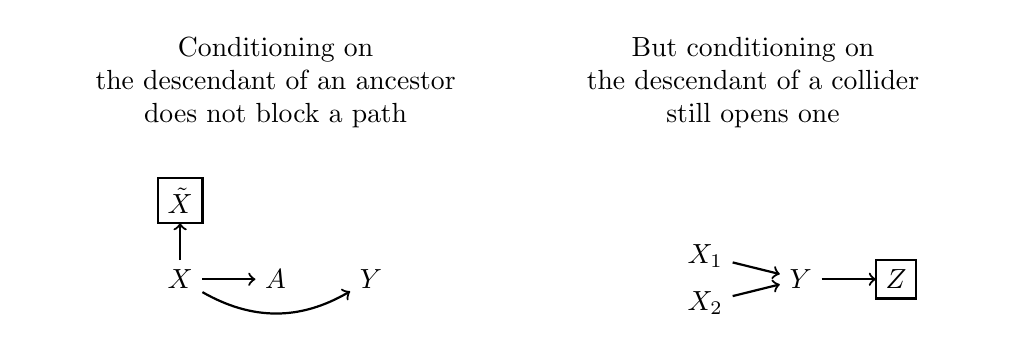
\begin{tikzpicture}[x = \textwidth]
\node at (0,0) {};
\node at (1,0) {};
\node[align = center] at (.25,1) {Conditioning on\\the descendant of an ancestor\\does not block a path};
% ANCESTOR DAG
\node (x) at (.15,-1.5) {$X$};
\node (xtilde) at (.15,-.5) {$\tilde{X}$};
\node (a) at (.25,-1.5) {$A$};
\node (ya) at (.35,-1.5) {$Y$};
\draw[thick] (xtilde.south west) rectangle (xtilde.north east);
\draw[->, thick] (x) -- (a);
\draw[->, thick] (x) -- (xtilde);
\draw[->, thick] (x) to[bend right] (ya); \pause
% COLLIDER DAG
\node[align = center] at (.75,1) {But conditioning on\\the descendant of a collider\\still opens one};
\node (x1) at (.7,-1.2) {$X_1$};
\node (yc) at (.8,-1.5) {$Y$};
\node (x3) at (.7,-1.8) {$X_2$};
\node (z) at (.9,-1.5) {$Z$};
\draw[thick] (z.south west) rectangle (z.north east);
\draw[->, thick] (x1) -- (yc);
\draw[->, thick] (x3) -- (yc);
\draw[->, thick] (yc) -- (z);
\end{tikzpicture}

\end{frame}

\begin{frame}{d-separation: Formal definition of blocking backdoor paths}
From Greenland, Pearl, \& Robins 1999, p. 45: \vskip .2in
\begin{quote}
...we say that a set of variables $S$ \emph{separates} two other sets $R$ and $T$, or $S$ \emph{blocks} every path between $R$ and $T$, if the following criteria are met:
\begin{enumerate}
\item Every unblocked path from $R$ to $T$ is intercepted by a variable in $S$, and
\item Every unblocked path from $R$ to $T$ generated by adjustment for the variables in $S$ is intercepted by a variable in $S$
\end{enumerate}
(This concept is usually called ``$d$-separation of $R$ and $T$ by $S$'' in the graphical literature, where $d$ stands for ``directional.''
\end{quote} \vskip .1in
Intuition: $R\leftarrow \boxed{S}\rightarrow T$
\end{frame}

\begin{frame}{Exercise}
Find 3 sufficient adjustment sets to identify $A\rightarrow Y$ \vskip .2in
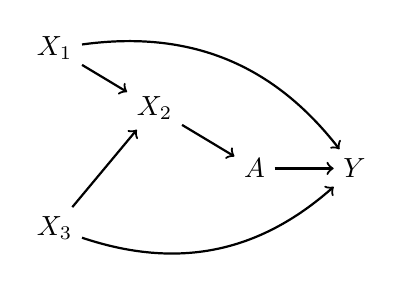
\begin{tikzpicture}[x = .5in, y = .3in]
\node (x1) at (-2,2) {$X_1$};
\node (x2) at (-1,1) {$X_2$};
\node (a) at (0,0) {$A$};
\node (y) at (1,0) {$Y$};
\node (x3) at (-2,-1) {$X_3$};
\draw[->, thick] (a) -- (y);
\draw[->, thick] (x1) -- (x2);
\draw[->, thick] (x1) to[bend left] (y);
\draw[->, thick] (x2) -- (a);
\draw[->, thick] (x3) -- (x2);
\draw[->, thick] (x3) to[bend right] (y);
\end{tikzpicture} \vskip .2in \pause
Answer: $\{X_2\},\{X_1,X_3\},\{X_1,X_2,X_3\}$

\end{frame}

\begin{frame}{Exercise}
What is the smallest adjustment set that identifies $A\rightarrow Y$? \vskip .2in
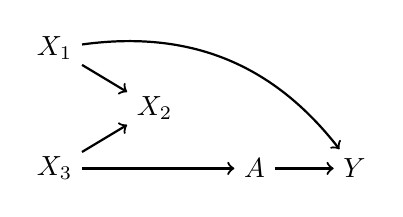
\begin{tikzpicture}[x = .5in, y = .3in]
\node (x1) at (-2,2) {$X_1$};
\node (x2) at (-1,1) {$X_2$};
\node (a) at (0,0) {$A$};
\node (y) at (1,0) {$Y$};
\node (x3) at (-2,0) {$X_3$};
\draw[->, thick] (a) -- (y);
\draw[->, thick] (x1) -- (x2);
\draw[->, thick] (x1) to[bend left] (y);
\draw[->, thick] (x3) -- (x2);
\draw[->, thick] (x3) -- (a);
\end{tikzpicture} \vskip .2in \pause
\begin{tabular}{ll}
\bgray{Answer:}& The empty set! Don't condition on anything.\\
&The collider $X_2$ already blocks the path.
\end{tabular}
\end{frame}

\begin{frame}{Key Concept: DAGs are better than rules of thumb}

\begin{tikzpicture}[x = \textwidth, y = .8\textheight]
\node at (0,0) {};
\node at (1,1) {};
\onslide<2->{
\node[anchor= north west] at (0,1) {Incorrect Rule of Thumb:};
\node[anchor= north west, align = left] at (.1,.92) {Adjust for all variables that are related to the treatment\\and related to the outcome.};
}
\node<3-9>[anchor= north west, align = left] at (0,.75) {Examples where that rule fails:};
\onslide<4-5>{
\node (a) at (.3, .45) {$A$};
\node (m) at (.5, .6) {$M$};
\node (y) at (.7, .45) {$Y$};
\draw[->, thick] (a) -- (m);
\draw[->, thick] (a) -- (y);
\draw[->, thick] (m) -- (y);
\node[anchor = west] at (0,.35) {--- $M$ is related to $A$};
\node[anchor = west] at (0,.28) {--- $M$ is related to $Y$};
}
\onslide<5>{
\node[anchor = west] at (0,.21) {--- But conditioning on $M$ blocks a causal path!};
\node[anchor = south west, font = \tiny, align = left, text width = \textwidth] at (0,0) {Imai, K., Keele, L., Tingley, D., \& Yamamoto, T. (2011). Unpacking the black box of causality: Learning about causal mechanisms from experimental and observational studies. American Political Science Review, 105(4), 765-789.};
}
\onslide<6-7>{
\node (a) at (.5, .45) {$A$};
\node (u1) at (.25, .6) {$U_1$};
\node (x) at (.4, .525) {$X$};
\node (u2) at (.25, .45) {$U_2$};
\node (y) at (.7, .45) {$Y$};
\draw[->, thick] (u1) to[out = 0, in = 135] (y);
\draw[->, thick] (u1) -- (x);
\draw[->, thick] (u2) -- (x);
\draw[->, thick] (u2) -- (a);
\draw[->, thick] (a) -- (y);
\node[anchor = west] at (0,.35) {--- $X$ is related to $A$};
\node[anchor = west] at (0,.28) {--- $X$ is related to $Y$};
}
\onslide<7>{
\node[anchor = west] at (0,.21) {--- But conditioning on $X$ opens the backdoor path!};
\node[anchor = south west, font = \tiny, align = left, text width = \textwidth] at (0,0) {Greenland, S. (2003). Quantifying biases in causal models: classical confounding vs collider-stratification bias. Epidemiology, 14(3), 300-306.};
}
\onslide<8-9>{
\node (a) at (.5, .45) {$A$};
\node (u) at (.6, .6) {$U$};
\node (z) at (.3, .45) {$Z$};
\node (y) at (.7, .45) {$Y$};
\draw[->, thick] (u) -- (y);
\draw[->, thick] (u) -- (a);
\draw[->, thick] (z) -- (a);
\draw[->, thick] (a) -- (y);
\node[anchor = west] at (0,.35) {--- $Z$ is related to $A$};
\node[anchor = west] at (0,.28) {--- $Z$ is related to $Y$, given $A$};
}
\onslide<9>{
\node[anchor = west] at (0,.21) {--- But conditioning on $Z$ amplifies bias from $U$!};
\node[anchor = south west, font = \tiny, align = left, text width = \textwidth] at (0,0) {Pearl, J. (2011). Invited commentary: Understanding bias amplification. American Journal of Epidemiology, 174(11), 1223-1227.};
}
\node<10->[anchor= north west, align = center, font = \large] at (0,.73) {The rule of thumb commits a \bgray{fundamental error}.};
\node<11->[anchor= north west, align = center, font = \large] at (0,.63) {It presents a criterion that is};
\node<11->[anchor= north, align = center, font = \huge] at (.5,.56) {statistical};
\node<11->[anchor= north, align = center, font = \large] at (.5,.47) {(involving observed relationships among variables)};
\node<12->[anchor= north west, align = center, font = \large] at (0,.33) {when we need a criterion that is};
\node<12->[anchor= north, align = center, font = \huge] at (.5,.26) {causal};
\node<12->[anchor= north, align = center, font = \large] at (.5,.17) {(involving counterfactual values)};
\node<13->[anchor= south west, align = center, font = \large] at (0,0) {This is why we need a DAG.};
\end{tikzpicture}

\end{frame}

\goalsframe

\begin{frame}{Let me know what you are thinking}

\begin{huge} \bref{https://tinyurl.com/CausalQuestions}{tinyurl.com/CausalQuestions} \end{huge}
\vskip .7in

Office hours TTh 11am-12pm and at \bref{https://calendly.com/ianlundberg/office-hours}{calendly.com/ianlundberg/office-hours}\\Come say hi!

\end{frame}

\end{document}




